\documentclass[twoside]{book}

% Packages required by doxygen
\usepackage{fixltx2e}
\usepackage{calc}
\usepackage{doxygen}
\usepackage[export]{adjustbox} % also loads graphicx
\usepackage{graphicx}
\usepackage[utf8]{inputenc}
\usepackage{makeidx}
\usepackage{multicol}
\usepackage{multirow}
\PassOptionsToPackage{warn}{textcomp}
\usepackage{textcomp}
\usepackage[nointegrals]{wasysym}
\usepackage[table]{xcolor}

% Font selection
\usepackage[T1]{fontenc}
\usepackage[scaled=.90]{helvet}
\usepackage{courier}
\usepackage{amssymb}
\usepackage{sectsty}
\renewcommand{\familydefault}{\sfdefault}
\allsectionsfont{%
  \fontseries{bc}\selectfont%
  \color{darkgray}%
}
\renewcommand{\DoxyLabelFont}{%
  \fontseries{bc}\selectfont%
  \color{darkgray}%
}
\newcommand{\+}{\discretionary{\mbox{\scriptsize$\hookleftarrow$}}{}{}}

% Page & text layout
\usepackage{geometry}
\geometry{%
  a4paper,%
  top=2.5cm,%
  bottom=2.5cm,%
  left=2.5cm,%
  right=2.5cm%
}
\tolerance=750
\hfuzz=15pt
\hbadness=750
\setlength{\emergencystretch}{15pt}
\setlength{\parindent}{0cm}
\setlength{\parskip}{3ex plus 2ex minus 2ex}
\makeatletter
\renewcommand{\paragraph}{%
  \@startsection{paragraph}{4}{0ex}{-1.0ex}{1.0ex}{%
    \normalfont\normalsize\bfseries\SS@parafont%
  }%
}
\renewcommand{\subparagraph}{%
  \@startsection{subparagraph}{5}{0ex}{-1.0ex}{1.0ex}{%
    \normalfont\normalsize\bfseries\SS@subparafont%
  }%
}
\makeatother

% Headers & footers
\usepackage{fancyhdr}
\pagestyle{fancyplain}
\fancyhead[LE]{\fancyplain{}{\bfseries\thepage}}
\fancyhead[CE]{\fancyplain{}{}}
\fancyhead[RE]{\fancyplain{}{\bfseries\leftmark}}
\fancyhead[LO]{\fancyplain{}{\bfseries\rightmark}}
\fancyhead[CO]{\fancyplain{}{}}
\fancyhead[RO]{\fancyplain{}{\bfseries\thepage}}
\fancyfoot[LE]{\fancyplain{}{}}
\fancyfoot[CE]{\fancyplain{}{}}
\fancyfoot[RE]{\fancyplain{}{\bfseries\scriptsize Generated by Doxygen }}
\fancyfoot[LO]{\fancyplain{}{\bfseries\scriptsize Generated by Doxygen }}
\fancyfoot[CO]{\fancyplain{}{}}
\fancyfoot[RO]{\fancyplain{}{}}
\renewcommand{\footrulewidth}{0.4pt}
\renewcommand{\chaptermark}[1]{%
  \markboth{#1}{}%
}
\renewcommand{\sectionmark}[1]{%
  \markright{\thesection\ #1}%
}

% Indices & bibliography
\usepackage{natbib}
\usepackage[titles]{tocloft}
\setcounter{tocdepth}{3}
\setcounter{secnumdepth}{5}
\makeindex

% Hyperlinks (required, but should be loaded last)
\usepackage{ifpdf}
\ifpdf
  \usepackage[pdftex,pagebackref=true]{hyperref}
\else
  \usepackage[ps2pdf,pagebackref=true]{hyperref}
\fi
\hypersetup{%
  colorlinks=true,%
  linkcolor=blue,%
  citecolor=blue,%
  unicode%
}

% Custom commands
\newcommand{\clearemptydoublepage}{%
  \newpage{\pagestyle{empty}\cleardoublepage}%
}

\usepackage{caption}
\captionsetup{labelsep=space,justification=centering,font={bf},singlelinecheck=off,skip=4pt,position=top}

%===== C O N T E N T S =====

\begin{document}

% Titlepage & ToC
\hypersetup{pageanchor=false,
             bookmarksnumbered=true,
             pdfencoding=unicode
            }
\pagenumbering{roman}
\begin{titlepage}
\vspace*{7cm}
\begin{center}%
{\Large My Project }\\
\vspace*{1cm}
{\large Generated by Doxygen 1.8.11}\\
\end{center}
\end{titlepage}
\clearemptydoublepage
\tableofcontents
\clearemptydoublepage
\pagenumbering{arabic}
\hypersetup{pageanchor=true}

%--- Begin generated contents ---
\chapter{Data Structure Index}
\section{Data Structures}
Here are the data structures with brief descriptions\+:\begin{DoxyCompactList}
\item\contentsline{section}{\hyperlink{structcamera}{camera} }{\pageref{structcamera}}{}
\item\contentsline{section}{\hyperlink{structenigme}{enigme} }{\pageref{structenigme}}{}
\item\contentsline{section}{\hyperlink{structperso}{perso} }{\pageref{structperso}}{}
\end{DoxyCompactList}

\chapter{File Index}
\section{File List}
Here is a list of all documented files with brief descriptions\+:\begin{DoxyCompactList}
\item\contentsline{section}{\hyperlink{ajoutconditions_8c}{ajoutconditions.\+c} \\*Ajouter conditions }{\pageref{ajoutconditions_8c}}{}
\item\contentsline{section}{\hyperlink{enigme_8c}{enigme.\+c} \\*Resolution enigme }{\pageref{enigme_8c}}{}
\item\contentsline{section}{{\bfseries enigme.\+h} }{\pageref{enigme_8h}}{}
\end{DoxyCompactList}

\chapter{Data Structure Documentation}
\hypertarget{structcamera}{}\section{camera Struct Reference}
\label{structcamera}\index{camera@{camera}}
\subsection*{Data Fields}
\begin{DoxyCompactItemize}
\item 
S\+D\+L\+\_\+\+Rect {\bfseries posdT}\hypertarget{structcamera_a009926b7b18bd483f27645f463f7463c}{}\label{structcamera_a009926b7b18bd483f27645f463f7463c}

\item 
S\+D\+L\+\_\+\+Rect {\bfseries p\+XR}\hypertarget{structcamera_ae3a1e769fbfe10ea4d1453c16c42e3ce}{}\label{structcamera_ae3a1e769fbfe10ea4d1453c16c42e3ce}

\item 
S\+D\+L\+\_\+\+Rect {\bfseries c\+XR}\hypertarget{structcamera_a134fe062710ef10c8aa37628c9fbe1f5}{}\label{structcamera_a134fe062710ef10c8aa37628c9fbe1f5}

\item 
double {\bfseries F\+PS}\hypertarget{structcamera_afea4555da34258956a5c18694a620d68}{}\label{structcamera_afea4555da34258956a5c18694a620d68}

\item 
int {\bfseries dT}\hypertarget{structcamera_a8b299ba58c00e93ad02d6bdbad871d9f}{}\label{structcamera_a8b299ba58c00e93ad02d6bdbad871d9f}

\item 
double {\bfseries Frm\+Strt}\hypertarget{structcamera_a62f48b9a8e4a2adb44fd95a80b4ff5d7}{}\label{structcamera_a62f48b9a8e4a2adb44fd95a80b4ff5d7}

\item 
double {\bfseries Frm\+End}\hypertarget{structcamera_a0689e8f79e69ab9bc91c1be2e4a66ea3}{}\label{structcamera_a0689e8f79e69ab9bc91c1be2e4a66ea3}

\item 
char {\bfseries DT} \mbox{[}50\mbox{]}\hypertarget{structcamera_a754156e5c7401a783f4a0e4a8917c1fd}{}\label{structcamera_a754156e5c7401a783f4a0e4a8917c1fd}

\item 
S\+D\+L\+\_\+\+Rect {\bfseries cam}\hypertarget{structcamera_a3edd8c2acc4df627823502ae4728355d}{}\label{structcamera_a3edd8c2acc4df627823502ae4728355d}

\item 
char {\bfseries camX} \mbox{[}50\mbox{]}\hypertarget{structcamera_a1bf016767b358b1d76be4ef77fb3d861}{}\label{structcamera_a1bf016767b358b1d76be4ef77fb3d861}

\end{DoxyCompactItemize}


The documentation for this struct was generated from the following file\+:\begin{DoxyCompactItemize}
\item 
\hyperlink{ajoutconditions_8c}{ajoutconditions.\+c}\end{DoxyCompactItemize}

\hypertarget{structenigme}{}\section{enigme Struct Reference}
\label{structenigme}\index{enigme@{enigme}}
\subsection*{Data Fields}
\begin{DoxyCompactItemize}
\item 
S\+D\+L\+\_\+\+Surface $\ast$ {\bfseries fond}\hypertarget{structenigme_a0a53a21d5fa8a66dd6cece93a3d4dedf}{}\label{structenigme_a0a53a21d5fa8a66dd6cece93a3d4dedf}

\item 
F\+I\+LE $\ast$ {\bfseries f}\hypertarget{structenigme_a9ce33d500de045fd29a8aa61c2fc0e1f}{}\label{structenigme_a9ce33d500de045fd29a8aa61c2fc0e1f}

\item 
S\+D\+L\+\_\+\+Rect {\bfseries posquest}\hypertarget{structenigme_af4f18b05a7c628d40ab10f318304b213}{}\label{structenigme_af4f18b05a7c628d40ab10f318304b213}

\item 
S\+D\+L\+\_\+\+Rect {\bfseries posr1}\hypertarget{structenigme_a198924786e9a05bb5b4d04ad8d43ac86}{}\label{structenigme_a198924786e9a05bb5b4d04ad8d43ac86}

\item 
S\+D\+L\+\_\+\+Rect {\bfseries posr2}\hypertarget{structenigme_a50cec981a8a981b124aa557032ea496b}{}\label{structenigme_a50cec981a8a981b124aa557032ea496b}

\item 
S\+D\+L\+\_\+\+Rect {\bfseries posr3}\hypertarget{structenigme_aa0b8e48586298a048a456976e0f76768}{}\label{structenigme_aa0b8e48586298a048a456976e0f76768}

\item 
S\+D\+L\+\_\+\+Rect {\bfseries posimageo}\hypertarget{structenigme_aa9ff126088547313032bbef03b551e02}{}\label{structenigme_aa9ff126088547313032bbef03b551e02}

\item 
S\+D\+L\+\_\+\+Rect {\bfseries posimagen}\hypertarget{structenigme_a343a7b9c26e6fc879f8fc2a2a13af6ec}{}\label{structenigme_a343a7b9c26e6fc879f8fc2a2a13af6ec}

\item 
S\+D\+L\+\_\+\+Surface {\bfseries imageo}\hypertarget{structenigme_ab44163a8aa438b4b2cf3d2f5be37d673}{}\label{structenigme_ab44163a8aa438b4b2cf3d2f5be37d673}

\item 
S\+D\+L\+\_\+\+Surface {\bfseries imagen}\hypertarget{structenigme_a05ed865cfa70da5d32cc9a717d6e2ad2}{}\label{structenigme_a05ed865cfa70da5d32cc9a717d6e2ad2}

\item 
S\+D\+L\+\_\+\+Rect {\bfseries pr1}\hypertarget{structenigme_a7eb8d641d45e4335b2c60b2a0c9037b8}{}\label{structenigme_a7eb8d641d45e4335b2c60b2a0c9037b8}

\item 
S\+D\+L\+\_\+\+Rect {\bfseries pr2}\hypertarget{structenigme_a89804b27f3bedda2234d71fb1ef88d5c}{}\label{structenigme_a89804b27f3bedda2234d71fb1ef88d5c}

\item 
S\+D\+L\+\_\+\+Rect {\bfseries pr3}\hypertarget{structenigme_ab6d9edd0a3901773473fd915ae966c4e}{}\label{structenigme_ab6d9edd0a3901773473fd915ae966c4e}

\item 
S\+D\+L\+\_\+\+Rect {\bfseries pv}\hypertarget{structenigme_a8519c7f181a11df67997195efb238b2c}{}\label{structenigme_a8519c7f181a11df67997195efb238b2c}

\item 
S\+D\+L\+\_\+\+Rect {\bfseries pquest}\hypertarget{structenigme_af12cfbe9e843ffbbd612c9bcc44921df}{}\label{structenigme_af12cfbe9e843ffbbd612c9bcc44921df}

\item 
S\+D\+L\+\_\+\+Rect {\bfseries positionimageo}\hypertarget{structenigme_a39d4b9366ba7e1b12c86b566f2cfdb99}{}\label{structenigme_a39d4b9366ba7e1b12c86b566f2cfdb99}

\item 
S\+D\+L\+\_\+\+Rect {\bfseries positionimagen}\hypertarget{structenigme_a0ec54db450f29c0170467f3718902f3c}{}\label{structenigme_a0ec54db450f29c0170467f3718902f3c}

\item 
char {\bfseries quest} \mbox{[}400\mbox{]}\hypertarget{structenigme_af85395df667ca31b4da0b9e45042658f}{}\label{structenigme_af85395df667ca31b4da0b9e45042658f}

\item 
char {\bfseries r1} \mbox{[}50\mbox{]}\hypertarget{structenigme_ab8ad9d1dd77fd405f1a4902afb556ba9}{}\label{structenigme_ab8ad9d1dd77fd405f1a4902afb556ba9}

\item 
char {\bfseries r2} \mbox{[}50\mbox{]}\hypertarget{structenigme_a69e2c99402f8552d706889398269fb02}{}\label{structenigme_a69e2c99402f8552d706889398269fb02}

\item 
char {\bfseries r3} \mbox{[}50\mbox{]}\hypertarget{structenigme_a0be499a1cab137aeaa3d66f50943519a}{}\label{structenigme_a0be499a1cab137aeaa3d66f50943519a}

\item 
char {\bfseries v} \mbox{[}50\mbox{]}\hypertarget{structenigme_a70d8de7b09d42617367d49020d219dc8}{}\label{structenigme_a70d8de7b09d42617367d49020d219dc8}

\end{DoxyCompactItemize}


The documentation for this struct was generated from the following file\+:\begin{DoxyCompactItemize}
\item 
enigme.\+h\end{DoxyCompactItemize}

\hypertarget{structperso}{}\section{perso Struct Reference}
\label{structperso}\index{perso@{perso}}
\subsection*{Data Fields}
\begin{DoxyCompactItemize}
\item 
S\+D\+L\+\_\+\+Surface $\ast$ {\bfseries image2}\hypertarget{structperso_a62acbc115de845349106a28c73f93aea}{}\label{structperso_a62acbc115de845349106a28c73f93aea}

\item 
S\+D\+L\+\_\+\+Rect {\bfseries pos\+Player}\hypertarget{structperso_aa36fa83b86aac6e58217acdf83f1d1b0}{}\label{structperso_aa36fa83b86aac6e58217acdf83f1d1b0}

\item 
int {\bfseries done}\hypertarget{structperso_a27424a1bed94325802586e357d724d4c}{}\label{structperso_a27424a1bed94325802586e357d724d4c}

\item 
int {\bfseries right}\hypertarget{structperso_a659a8d5f2ffd70918846dd53fd14c04f}{}\label{structperso_a659a8d5f2ffd70918846dd53fd14c04f}

\item 
int {\bfseries left}\hypertarget{structperso_a09b35ffe6af078416f3f9400963764b1}{}\label{structperso_a09b35ffe6af078416f3f9400963764b1}

\item 
int {\bfseries sprint}\hypertarget{structperso_ac0f658e9861cbd772d809d0b8a4527f5}{}\label{structperso_ac0f658e9861cbd772d809d0b8a4527f5}

\item 
int {\bfseries maxspeed}\hypertarget{structperso_ace2be8d984c92ac5bc862c4fae73ccd8}{}\label{structperso_ace2be8d984c92ac5bc862c4fae73ccd8}

\item 
double {\bfseries x\+Vel}\hypertarget{structperso_a72bb6943583c5a7b55639cf164e00677}{}\label{structperso_a72bb6943583c5a7b55639cf164e00677}

\item 
double {\bfseries y\+Vel}\hypertarget{structperso_a4bee30ab165fd9910d8090bcd1d2342d}{}\label{structperso_a4bee30ab165fd9910d8090bcd1d2342d}

\item 
double {\bfseries can\+Jump}\hypertarget{structperso_a9149a0b708d69657fc271ade4cbbb431}{}\label{structperso_a9149a0b708d69657fc271ade4cbbb431}

\item 
double {\bfseries v\+\_\+jump}\hypertarget{structperso_a26ad027d7b76973535e7969482725da6}{}\label{structperso_a26ad027d7b76973535e7969482725da6}

\item 
double {\bfseries gravity}\hypertarget{structperso_a4c95e3d16f0d4eae52c1187d6ddfd573}{}\label{structperso_a4c95e3d16f0d4eae52c1187d6ddfd573}

\item 
int {\bfseries acc}\hypertarget{structperso_a1a32aa71194817603bd160c2b9cbf197}{}\label{structperso_a1a32aa71194817603bd160c2b9cbf197}

\item 
int {\bfseries ianim}\hypertarget{structperso_a4674f7d91c33283d7b7e7772fb00de13}{}\label{structperso_a4674f7d91c33283d7b7e7772fb00de13}

\item 
int {\bfseries ianim\+\_\+c}\hypertarget{structperso_afe1ee12c60466189e822f1edff0c49b1}{}\label{structperso_afe1ee12c60466189e822f1edff0c49b1}

\item 
int {\bfseries timer}\hypertarget{structperso_ab032e3ba9ddeb4e51ff9a6c2ccfc6974}{}\label{structperso_ab032e3ba9ddeb4e51ff9a6c2ccfc6974}

\item 
int {\bfseries maxtimer}\hypertarget{structperso_a17c1c31df790c449d6ca2745479caf9d}{}\label{structperso_a17c1c31df790c449d6ca2745479caf9d}

\item 
char {\bfseries playerX} \mbox{[}50\mbox{]}\hypertarget{structperso_ae3fc2ec8c3c4467de79660c795df383d}{}\label{structperso_ae3fc2ec8c3c4467de79660c795df383d}

\item 
char {\bfseries animchar} \mbox{[}50\mbox{]}\hypertarget{structperso_aefd47a77481e0495003239f70c62a829}{}\label{structperso_aefd47a77481e0495003239f70c62a829}

\item 
T\+T\+F\+\_\+\+Font $\ast$ {\bfseries textF}\hypertarget{structperso_afce99f59fe877aaceae0279e4c4b35a2}{}\label{structperso_afce99f59fe877aaceae0279e4c4b35a2}

\end{DoxyCompactItemize}


The documentation for this struct was generated from the following file\+:\begin{DoxyCompactItemize}
\item 
\hyperlink{ajoutconditions_8c}{ajoutconditions.\+c}\end{DoxyCompactItemize}

\chapter{File Documentation}
\hypertarget{ajoutconditions_8c}{}\section{ajoutconditions.\+c File Reference}
\label{ajoutconditions_8c}\index{ajoutconditions.\+c@{ajoutconditions.\+c}}


ajouter conditions  


{\ttfamily \#include $<$S\+D\+L/\+S\+D\+L\+\_\+image.\+h$>$}\\*
{\ttfamily \#include $<$S\+D\+L/\+S\+D\+L\+\_\+ttf.\+h$>$}\\*
Include dependency graph for ajoutconditions.\+c\+:
\nopagebreak
\begin{figure}[H]
\begin{center}
\leavevmode
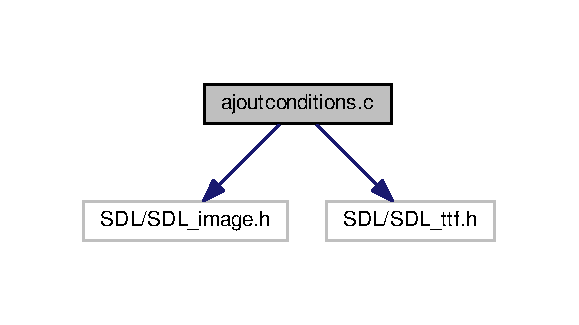
\includegraphics[width=278pt]{ajoutconditions_8c__incl}
\end{center}
\end{figure}
\subsection*{Data Structures}
\begin{DoxyCompactItemize}
\item 
struct \hyperlink{structperso}{perso}
\item 
struct \hyperlink{structcamera}{camera}
\end{DoxyCompactItemize}
\subsection*{Typedefs}
\begin{DoxyCompactItemize}
\item 
typedef struct \hyperlink{structperso}{perso} {\bfseries perso}\hypertarget{ajoutconditions_8c_a1c7a32a9b48d6f089882757a219edf09}{}\label{ajoutconditions_8c_a1c7a32a9b48d6f089882757a219edf09}

\item 
typedef struct \hyperlink{structcamera}{camera} {\bfseries camera}\hypertarget{ajoutconditions_8c_ae26b36add9a7cd89501e76cd66317f5c}{}\label{ajoutconditions_8c_ae26b36add9a7cd89501e76cd66317f5c}

\end{DoxyCompactItemize}
\subsection*{Functions}
\begin{DoxyCompactItemize}
\item 
void {\bfseries ajoutconditions} (int vie, int coeur, int niveau, int score, S\+D\+L\+\_\+\+Surface $\ast$ecran)\hypertarget{ajoutconditions_8c_a934514ef2c799fb64861419047f1aefb}{}\label{ajoutconditions_8c_a934514ef2c799fb64861419047f1aefb}

\item 
void \hyperlink{ajoutconditions_8c_ad0b3e665125a6aaf7ce1cdb425941845}{initialiserpersos} (\hyperlink{structperso}{perso} $\ast$p)
\begin{DoxyCompactList}\small\item\em initialiser personnage \end{DoxyCompactList}\item 
void \hyperlink{ajoutconditions_8c_a675a6d1471d4fc75b830c83b08434d01}{initialiserpersof} (\hyperlink{structperso}{perso} $\ast$p)
\begin{DoxyCompactList}\small\item\em initialiser personnage \end{DoxyCompactList}\item 
void \hyperlink{ajoutconditions_8c_afec174ec74fa4a1e39000b472eb8a2c7}{ajoutpersonnage} (\hyperlink{structperso}{perso} $\ast$p)
\begin{DoxyCompactList}\small\item\em ajouter personnage \end{DoxyCompactList}\end{DoxyCompactItemize}


\subsection{Detailed Description}
ajouter conditions 


\begin{DoxyParams}{Parameters}
{\em entier} & vie \\
\hline
{\em entier} & coeur \\
\hline
{\em entier} & niveau \\
\hline
{\em entier} & score \\
\hline
{\em ecran} & image \\
\hline
\end{DoxyParams}
\begin{DoxyReturn}{Returns}
nothing 
\end{DoxyReturn}


\subsection{Function Documentation}
\index{ajoutconditions.\+c@{ajoutconditions.\+c}!ajoutpersonnage@{ajoutpersonnage}}
\index{ajoutpersonnage@{ajoutpersonnage}!ajoutconditions.\+c@{ajoutconditions.\+c}}
\subsubsection[{\texorpdfstring{ajoutpersonnage(perso $\ast$p)}{ajoutpersonnage(perso *p)}}]{\setlength{\rightskip}{0pt plus 5cm}void ajoutpersonnage (
\begin{DoxyParamCaption}
\item[{{\bf perso} $\ast$}]{p}
\end{DoxyParamCaption}
)}\hypertarget{ajoutconditions_8c_afec174ec74fa4a1e39000b472eb8a2c7}{}\label{ajoutconditions_8c_afec174ec74fa4a1e39000b472eb8a2c7}


ajouter personnage 


\begin{DoxyParams}{Parameters}
{\em struct} & perso \\
\hline
\end{DoxyParams}
\begin{DoxyReturn}{Returns}
nothing 
\end{DoxyReturn}


Here is the call graph for this function\+:
\nopagebreak
\begin{figure}[H]
\begin{center}
\leavevmode
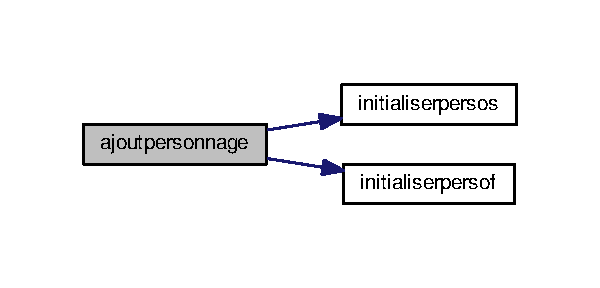
\includegraphics[width=288pt]{ajoutconditions_8c_afec174ec74fa4a1e39000b472eb8a2c7_cgraph}
\end{center}
\end{figure}


\index{ajoutconditions.\+c@{ajoutconditions.\+c}!initialiserpersof@{initialiserpersof}}
\index{initialiserpersof@{initialiserpersof}!ajoutconditions.\+c@{ajoutconditions.\+c}}
\subsubsection[{\texorpdfstring{initialiserpersof(perso $\ast$p)}{initialiserpersof(perso *p)}}]{\setlength{\rightskip}{0pt plus 5cm}void initialiserpersof (
\begin{DoxyParamCaption}
\item[{{\bf perso} $\ast$}]{p}
\end{DoxyParamCaption}
)}\hypertarget{ajoutconditions_8c_a675a6d1471d4fc75b830c83b08434d01}{}\label{ajoutconditions_8c_a675a6d1471d4fc75b830c83b08434d01}


initialiser personnage 


\begin{DoxyParams}{Parameters}
{\em struct} & perso \\
\hline
\end{DoxyParams}
\begin{DoxyReturn}{Returns}
nothing 
\end{DoxyReturn}


Here is the caller graph for this function\+:
\nopagebreak
\begin{figure}[H]
\begin{center}
\leavevmode
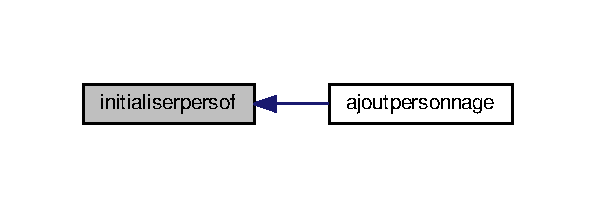
\includegraphics[width=286pt]{ajoutconditions_8c_a675a6d1471d4fc75b830c83b08434d01_icgraph}
\end{center}
\end{figure}


\index{ajoutconditions.\+c@{ajoutconditions.\+c}!initialiserpersos@{initialiserpersos}}
\index{initialiserpersos@{initialiserpersos}!ajoutconditions.\+c@{ajoutconditions.\+c}}
\subsubsection[{\texorpdfstring{initialiserpersos(perso $\ast$p)}{initialiserpersos(perso *p)}}]{\setlength{\rightskip}{0pt plus 5cm}void initialiserpersos (
\begin{DoxyParamCaption}
\item[{{\bf perso} $\ast$}]{p}
\end{DoxyParamCaption}
)}\hypertarget{ajoutconditions_8c_ad0b3e665125a6aaf7ce1cdb425941845}{}\label{ajoutconditions_8c_ad0b3e665125a6aaf7ce1cdb425941845}


initialiser personnage 


\begin{DoxyParams}{Parameters}
{\em struct} & perso \\
\hline
\end{DoxyParams}
\begin{DoxyReturn}{Returns}
nothing 
\end{DoxyReturn}


Here is the caller graph for this function\+:
\nopagebreak
\begin{figure}[H]
\begin{center}
\leavevmode
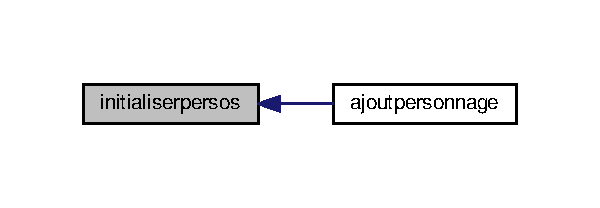
\includegraphics[width=288pt]{ajoutconditions_8c_ad0b3e665125a6aaf7ce1cdb425941845_icgraph}
\end{center}
\end{figure}



\hypertarget{enigme_8c}{}\section{enigme.\+c File Reference}
\label{enigme_8c}\index{enigme.\+c@{enigme.\+c}}


resolution enigme  


{\ttfamily \#include $<$stdio.\+h$>$}\\*
{\ttfamily \#include $<$stdlib.\+h$>$}\\*
{\ttfamily \#include \char`\"{}S\+D\+L/\+S\+D\+L.\+h\char`\"{}}\\*
{\ttfamily \#include \char`\"{}S\+D\+L/\+S\+D\+L\+\_\+image.\+h\char`\"{}}\\*
{\ttfamily \#include \char`\"{}S\+D\+L/\+S\+D\+L\+\_\+mixer.\+h\char`\"{}}\\*
{\ttfamily \#include \char`\"{}S\+D\+L/\+S\+D\+L\+\_\+ttf.\+h\char`\"{}}\\*
{\ttfamily \#include \char`\"{}enigme.\+h\char`\"{}}\\*
{\ttfamily \#include $<$time.\+h$>$}\\*
Include dependency graph for enigme.\+c\+:\nopagebreak
\begin{figure}[H]
\begin{center}
\leavevmode
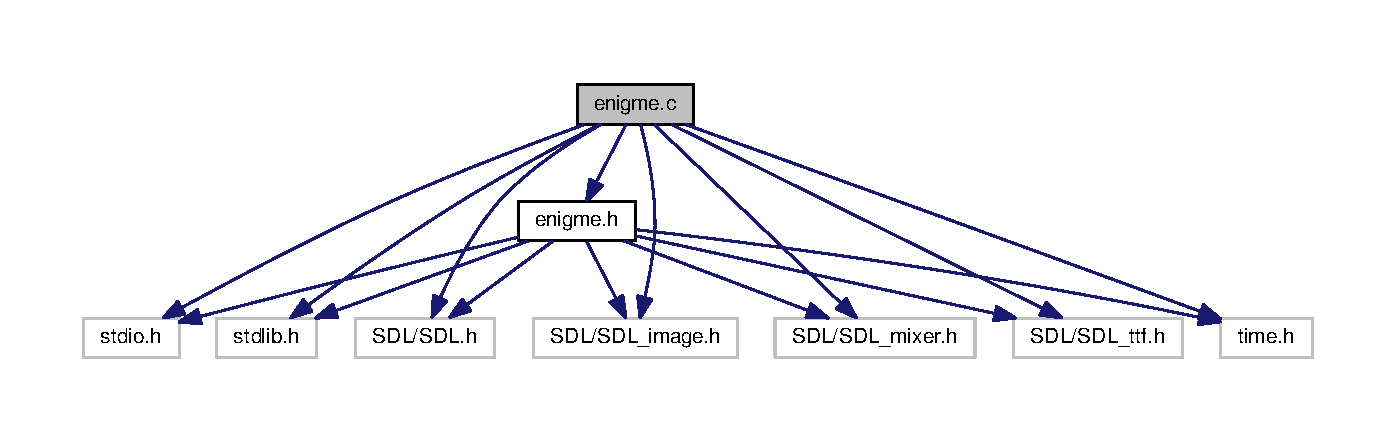
\includegraphics[width=350pt]{enigme_8c__incl}
\end{center}
\end{figure}
\subsection*{Functions}
\begin{DoxyCompactItemize}
\item 
int {\bfseries resolution\+Enigme} (enigmeg pe, \hyperlink{structenigme}{enigme} ed, S\+D\+L\+\_\+\+Event event)\hypertarget{enigme_8c_af1b0a446097e45b3ae1f2ffd9e716969}{}\label{enigme_8c_af1b0a446097e45b3ae1f2ffd9e716969}

\item 
void \hyperlink{enigme_8c_a647d93c077148cffedbc80eaafa7c1cb}{init\+Enigme} (\hyperlink{structenigme}{enigme} $\ast$e)
\begin{DoxyCompactList}\small\item\em initialisation enigme \end{DoxyCompactList}\item 
int \hyperlink{enigme_8c_a84e4437f43bda4dd8f4cabda651f8eb7}{random} ()
\begin{DoxyCompactList}\small\item\em random function \end{DoxyCompactList}\item 
\hyperlink{structenigme}{enigme} \hyperlink{enigme_8c_acbb0016ec6966abc952d0dd450804b39}{generer\+Enigme} (\hyperlink{structenigme}{enigme} e)
\begin{DoxyCompactList}\small\item\em generer enigme \end{DoxyCompactList}\end{DoxyCompactItemize}


\subsection{Detailed Description}
resolution enigme 


\begin{DoxyParams}{Parameters}
{\em e} & struct enigme \\
\hline
{\em event} & evenement \\
\hline
\end{DoxyParams}
\begin{DoxyReturn}{Returns}
1 if true 
\end{DoxyReturn}


\subsection{Function Documentation}
\index{enigme.\+c@{enigme.\+c}!generer\+Enigme@{generer\+Enigme}}
\index{generer\+Enigme@{generer\+Enigme}!enigme.\+c@{enigme.\+c}}
\subsubsection[{\texorpdfstring{generer\+Enigme(enigme e)}{genererEnigme(enigme e)}}]{\setlength{\rightskip}{0pt plus 5cm}{\bf enigme} generer\+Enigme (
\begin{DoxyParamCaption}
\item[{{\bf enigme}}]{e}
\end{DoxyParamCaption}
)}\hypertarget{enigme_8c_acbb0016ec6966abc952d0dd450804b39}{}\label{enigme_8c_acbb0016ec6966abc952d0dd450804b39}


generer enigme 


\begin{DoxyParams}{Parameters}
{\em e} & struct enigme \\
\hline
\end{DoxyParams}
\begin{DoxyReturn}{Returns}
struct enigme 
\end{DoxyReturn}


Here is the call graph for this function\+:\nopagebreak
\begin{figure}[H]
\begin{center}
\leavevmode
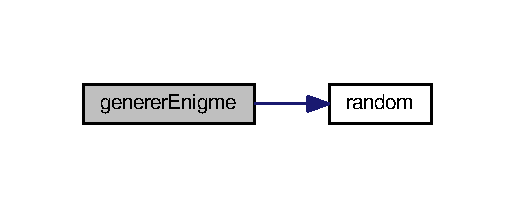
\includegraphics[width=247pt]{enigme_8c_acbb0016ec6966abc952d0dd450804b39_cgraph}
\end{center}
\end{figure}


\index{enigme.\+c@{enigme.\+c}!init\+Enigme@{init\+Enigme}}
\index{init\+Enigme@{init\+Enigme}!enigme.\+c@{enigme.\+c}}
\subsubsection[{\texorpdfstring{init\+Enigme(enigme $\ast$e)}{initEnigme(enigme *e)}}]{\setlength{\rightskip}{0pt plus 5cm}void init\+Enigme (
\begin{DoxyParamCaption}
\item[{{\bf enigme} $\ast$}]{e}
\end{DoxyParamCaption}
)}\hypertarget{enigme_8c_a647d93c077148cffedbc80eaafa7c1cb}{}\label{enigme_8c_a647d93c077148cffedbc80eaafa7c1cb}


initialisation enigme 


\begin{DoxyParams}{Parameters}
{\em $\ast$e} & struct enigme \\
\hline
\end{DoxyParams}
\begin{DoxyReturn}{Returns}
nothing 
\end{DoxyReturn}
\index{enigme.\+c@{enigme.\+c}!random@{random}}
\index{random@{random}!enigme.\+c@{enigme.\+c}}
\subsubsection[{\texorpdfstring{random()}{random()}}]{\setlength{\rightskip}{0pt plus 5cm}int random (
\begin{DoxyParamCaption}
{}
\end{DoxyParamCaption}
)}\hypertarget{enigme_8c_a84e4437f43bda4dd8f4cabda651f8eb7}{}\label{enigme_8c_a84e4437f43bda4dd8f4cabda651f8eb7}


random function 

\begin{DoxyReturn}{Returns}
entier 
\end{DoxyReturn}


Here is the caller graph for this function\+:\nopagebreak
\begin{figure}[H]
\begin{center}
\leavevmode
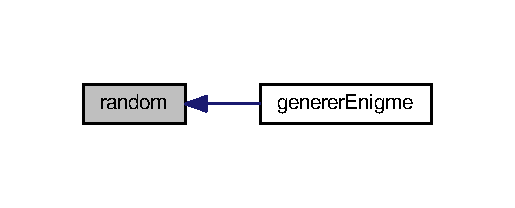
\includegraphics[width=247pt]{enigme_8c_a84e4437f43bda4dd8f4cabda651f8eb7_icgraph}
\end{center}
\end{figure}



%--- End generated contents ---

% Index
\backmatter
\newpage
\phantomsection
\clearemptydoublepage
\addcontentsline{toc}{chapter}{Index}
\printindex

\end{document}
